\chapter{Five Tips for Writing Your First Novel}

This lecture is not mathematical in the blackboard sense, but it is exact in another way. We begin with a numerical constraint, fifty thousand words in a month, and from that constraint Sanderson builds a sequence of practical constructions: borrow a structure, open a channel into a character, generate pressure from wants and needs, organize the whole story around progress, and then support the daily labor of writing by preparing the mind before we sit down. The order matters, because each step answers the insufficiency of the one before it.

\begin{remark}
No validated lecture screenshots survive for this chapter. The displayed formulas and the one schematic figure below are therefore transcript-led reconstructions, not transcriptions of visible board work.
\end{remark}

\section{Challenge, Permission, and the Five-Hack Setup}

We begin where Sanderson begins: with National Novel Writing Month as a practical challenge rather than a literary doctrine. The working target is a novel in one month, and the word novel is here defined loosely enough to support the challenge. Sanderson immediately notes that fifty thousand words is a rough operational number, not a theory of form; many of his own novels are much longer. But the challenge is still serious because it is both doable and difficult.

\begin{align}
\text{NaNoWriMo target} &= 50{,}000\ \text{words},\\
\text{daily pace} &\approx \frac{50{,}000}{30} \approx 1{,}667 \approx 1{,}700\ \text{words/day}.
\end{align}

The purpose of the exercise is equally important. We are meant to get out of a rut, to turn off the internal editor, and to write. Sanderson strengthens that claim by personal example: he did the challenge many times before publication, and even traces the original writing of \textit{The Way of Kings} back to such a month-long sprint. So the lecture begins not with abstraction but with a working constraint and a testimonial that the constraint can be productive.

Just as important, however, is the permission he gives almost at once. This may not work for every writer. The challenge may clash with a person's writing psychology, or the resulting pages may simply be worse than pages produced more slowly. That qualification sets the tone for the whole lecture. These are methods, not commandments.

\subsection{Question \& Answer}

\paragraph{Question.} When is this challenge useful, and when should we abandon it?

\paragraph{Answer.} It is useful when a hard external constraint helps us break hesitation, silence the internal editor, and accumulate pages. We should abandon it when the constraint stops serving the work, when it clearly fights our writing psychology, or when it makes the writing worse rather than freer.

Only after clearing that ground does Sanderson make the main promise of the talk: for those who do want to try, he will offer five hacks, five practical ways to start a novel even without much preparation.

\section{Borrowing Structure as Training Wheels}

The first hack begins with a familiar writerly impulse. We watch a film, read a story, hear about an event, and think: could we write something like that? Sanderson's answer is not to copy the story, but to analyze what in that kind of story is structurally alive. This does not happen with every novel and not with every writer, but when it does happen it can give us immediate traction.

\begin{definition}
A borrowed structure is the functional pattern of a story or subgenre, extracted from one instance and rebuilt with different characters, stakes, and arc.
\end{definition}

The lecture's clearest example is the heist. The attraction is not simply the criminal surface. It is the structure: a difficult problem, a set of complementary specialists, preparation, and a resolution in which those specializations must finally work together.

\begin{equation}
\text{admired story} \to \text{hallmark scenes} \to \text{fundamental structure} \to \text{new story}.
\end{equation}

In Sanderson's heist example, the structure can be compressed schematically as

\begin{equation}
\text{problem} \to \text{recruitment} \to \text{preparation} \to \text{coordinated resolution}.
\end{equation}

\paragraph{A worked extraction rule.} The lecture's method can be written as:
\begin{enumerate}
\item Start from a story or subgenre we admire.
\item Ask what makes that kind of story satisfying.
\item Extract the hallmark beats or scenes.
\item Boil those beats down to a fundamental structure.
\item Rebuild the structure with new characters, a new problem, and a new character arc.
\end{enumerate}

Once we see this, the structure comes loose from the original example. Sanderson reinforces the point by transposition: one may take a structure loved in Regency romance and move it into a Western. That shift preserves the skeleton while changing the flesh. It also prevents the borrowing from hardening into imitation.

\subsection{Question \& Answer}

\paragraph{Question.} How do we borrow a structure without becoming enslaved to it?

\paragraph{Answer.} We borrow the pattern, not the identity. The old story gives us a carrying sequence, but we replace its surface world, its characters, its central problem, and its arc. The borrowed structure serves as training wheels: real support, but not a permanent cage.

That last phrase is crucial. Sanderson says this can help enormously when we are trying to write quickly, yet he also insists that even professionals borrow structures in this way. So the method is not merely remedial; it is a legitimate way of stabilizing invention.

\section{Beginning with a Monologue}

Having supplied outer scaffolding, the lecture narrows from structure to access. How do we enter a character quickly enough to start writing? Sanderson's second answer is the monologue. Even if the finished novel will not be written as a first-person account, we can still ask a character to speak as if directly to us and explain some important part of life.

\begin{equation}
\text{monologue} \to \text{voice} + \text{history} + \text{usable fragments}.
\end{equation}

The point is discovery rather than final form. Sanderson gives the example of asking what a character would say if made to explain life in five pages. Those pages may never be printed in the finished novel. But they reveal diction, emphasis, memory, self-deception, and attitude. In that sense, the monologue is not addressed to the reader first; it is addressed to the writer.

The lecture then pushes the exercise one step further. Material generated this way may become epigraphs, journal fragments, or other small prefatory texts at the head of chapters. If the form proves especially fertile, it may even suggest a full epistolary novel.

\begin{definition}
An epistolary novel is a novel composed through in-world documents such as journals, letters, or similar writings.
\end{definition}

Sanderson's offhand description is useful here: this is in some sense the found-footage version of the novel. The analogy is loose, but it captures the formal idea quickly.

\subsection{Question \& Answer}

\paragraph{Question.} Can a first-person monologue be useful even when the finished novel is not first person?

\paragraph{Answer.} Yes. Here the monologue is not a doctrinal choice about viewpoint. It is a discovery device. We use it to hear the character, to extract voice and history, and only afterward do we decide what, if anything, survives into the finished book.

This is the lecture's second major pattern: a provisional exercise can remain provisional, but it may also yield finished material if the voice it produces turns out to be too valuable to discard.

\section{Wants, Needs, Obstacles, and Choosing the Right Viewpoint}

The third hack turns from voice to pressure. Sanderson asks four linked questions: what does the character want, what does the character need, how are those different, and why can the character have neither? At this point the lecture becomes structurally cleaner. Plot is no longer imposed from outside. It is generated from the misfit between conscious pursuit and deeper necessity.

Let us name the central quantities:
\begin{align}
W &= \text{what the character wants},\\
N &= \text{what the character needs},\\
O &= \text{the obstacles that block both}.
\end{align}

The crucial distinction is the nonidentity of the first two:

\begin{equation}
W \neq N.
\end{equation}

Once that split is in place, plot pressure follows:

\begin{equation}
\text{plot pressure} = \text{obstacles to } W \text{ and } N.
\end{equation}

\paragraph{A worked update rule.} Sanderson's procedure for generating plot from character can be compressed to:
\begin{enumerate}
\item Ask what the character wants.
\item Ask what the character needs.
\item Ask how those differ.
\item Ask why the character cannot simply have either one.
\item Turn the answers into obstacles.
\item Let those obstacles determine the early motion of the plot.
\end{enumerate}

This is why the lecture insists on a character-centered story. If the turns of the plot arise from the pressures around \(W\), \(N\), and \(O\), then the character remains inside the machinery of the novel rather than outside it.

From there Sanderson diagnoses a common beginner's mistake. We may choose the wrong viewpoint character: somebody who merely watches events while the true drama belongs to someone else. In that case the nominal protagonist becomes an external observer of a more interesting story.

\subsection{Question \& Answer}

\paragraph{Question.} Which character should actually carry the story?

\paragraph{Answer.} Not the passive observer. The story should belong to the character who is changing most, carrying the most conflict, or striving most actively for what is wanted. If another figure bears the real pressure, then that other figure is closer to the true protagonist.

The lecture uses this diagnosis as a bridge. Sanderson imagines the writer saying: all right, I now know what my character wants and needs, but I still do not have a structure. That complaint opens the way to the strongest formal passage in the talk.

\section{Promise, Progress, Payoff, and the Signposting of Motion}

The fourth hack is introduced explicitly as the answer to the structure objection. Sanderson says he has a whole lecture on the subject, but if he boils it down, stories are built from three ideas:

\begin{equation}
\text{story} = \text{promise} \to \text{progress} \to \text{payoff}.
\end{equation}

This triad deserves to stay near the center of the chapter. The promise names the kind of movement or satisfaction the story offers. The payoff fulfills that offer. But the large middle term, progress, is the bulk of the story. Readers keep turning pages because they can feel movement toward something.

Sanderson adds an unexpectedly useful observation here: even the physical shape of the book provides a coarse sense of progress. As pages pass, we are closer to the end. But that crude motion is not enough. The plot must reinforce it by giving us a more specific channel of advance.

\begin{figure}
\centering
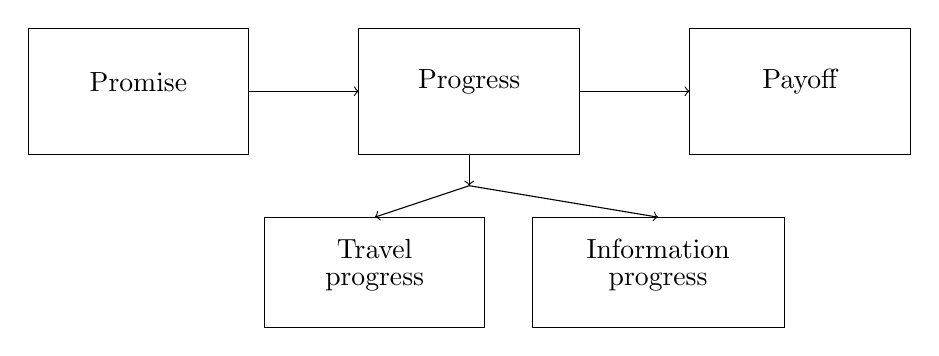
\begin{tikzpicture}
\draw (-5.2,0.8) rectangle (-2.4,-0.8);
\node at (-3.8,0.12) {Promise};

\draw (-1.0,0.8) rectangle (1.8,-0.8);
\node at (0.4,0.12) {Progress};

\draw (3.2,0.8) rectangle (6.0,-0.8);
\node at (4.6,0.12) {Payoff};

\draw[->] (-2.4,0) -- (-1.0,0);
\draw[->] (1.8,0) -- (3.2,0);

\draw (-2.2,-3.0) rectangle (0.6,-1.6);
\node at (-0.8,-2.0) {Travel};
\node at (-0.8,-2.42) {progress};

\draw (1.2,-3.0) rectangle (4.4,-1.6);
\node at (2.8,-2.0) {Information};
\node at (2.8,-2.42) {progress};

\draw[->] (0.4,-0.8) -- (0.4,-1.2);
\draw[->] (0.4,-1.2) -- (-0.8,-1.6);
\draw[->] (0.4,-1.2) -- (2.8,-1.6);
\end{tikzpicture}
\end{figure}

This is a transcript-only schematic. It does not claim visual backing from the lecture frames. It simply displays the distinction Sanderson makes between the general structure of story and the different channels along which progress can be measured.

His first example is geographic. In a quest we can measure motion by space:

\begin{equation}
\text{travel progress} : \text{start} \to \text{destination}.
\end{equation}

The lecture is careful not to equate progress with constant forward ease. Characters may be diverted, forced backward, or blocked from the route they expected. But those reversals remain legible because the destination remains stable enough to define what ``closer'' would mean.

The second example is informational. In a mystery the progress is not primarily spatial but epistemic:

\begin{equation}
\text{information progress} : \text{few clues} \to \text{more clues} \to \text{clearer picture}.
\end{equation}

False clues and wrong turns therefore do not destroy structure. They belong to it, provided the reader can still feel that the general image is sharpening.

From here Sanderson arrives at a diagnosis of pacing. A story may feel slow not because nothing occurs, but because the promised kind of progress is not being signposted clearly enough.

\begin{equation}
\text{signposted progress} \Rightarrow \text{page-turning momentum}.
\end{equation}

And the converse is equally important:

\begin{equation}
\text{misaligned signpost} \Rightarrow \text{perceived poor pacing}.
\end{equation}

\paragraph{Transcript note.} The transcript is rough in the lecture's example at this point, but the intended structural point is clear. If the story is signposted most strongly as an adventure while the writer is privately thinking of it as a romance, readers will measure progress on the adventure axis. They will then feel stasis if that promised channel is not being advanced.

\subsection{Question \& Answer}

\paragraph{Question.} Why does a story feel slow even when events are happening?

\paragraph{Answer.} Because events alone do not generate momentum. Momentum requires a visible progress channel. If we promise travel, the reader must feel spatial advance; if we promise a mystery, the reader must feel accumulating information. When that channel is weak or mismatched to the story's strongest signposts, the book feels static even while scenes are active.

Sanderson's final recommendation within this section is practical and exact: divide the larger channel of progress into smaller legible units, a trail of breadcrumbs, so that the reader can feel the motion locally as well as globally.

\section{Priming the Mind and Writing Ahead of the Page}

The fifth and final hack returns from the mechanics of story to the mechanics of work. If we are aiming at something like \(1{,}700\) words a day, we cannot afford to begin each session cold. Sanderson's solution is to prime the mind before the writing session itself.

\begin{equation}
\text{off-page rehearsal} \to \text{on-page execution}.
\end{equation}

The lecture is concrete about the kinds of time this means: commuting, working out, doing dishes, mowing the lawn, any activity that occupies the body while leaving the mind relatively free. Instead of allowing that time to dissipate, we may use it to ask what the next scene should do, what could make it vivid, and why it might become one of the book's memorable scenes.

\paragraph{A worked routine.} Sanderson's method can be summarized as:
\begin{enumerate}
\item Decide which scene is next.
\item Ask what must happen in it.
\item Ask what makes that scene interesting rather than routine.
\item Rehearse it mentally several times.
\item Sit down already knowing the next block of motion.
\end{enumerate}

He even adds a tonal refinement: music can help settle the imagination into the emotional register of the scene. The point is not ornament but reduced startup friction. By the time we reach the desk, the scene has already begun in the mind.

The lecture then generalizes the advice beyond the one-month challenge. Even if ordinary life leaves us only weekend writing time, off-page priming during the week can prepare those later hours. The final movement of the lecture is therefore structurally neat: after teaching us how to make a story move, Sanderson closes by teaching us how to keep the writer moving.

\section{Summary}

This lecture proceeds with more formal discipline than its casual tone first suggests. We begin with a numerical target and a permission structure: write quickly, turn off the internal editor, but do not worship the challenge if it works against your psychology. We then borrow outer structure, discover voice through monologue, generate plot from the tension between wants and needs, compress story into promise, progress, and payoff, and finally support the whole enterprise by thinking ahead of the page.

The chapter's central lesson is therefore procedural. A novel may be started under pressure if we stabilize invention with enough structure: an external constraint, a recoverable pattern, a character engine, a visible channel of progress, and a daily practice that reduces the gap between intention and execution. That is the order in which Sanderson leads us through the lecture, and it is the order that makes the notes feel like the lecture unfolding rather than a set of disconnected maxims.